\documentclass{jdrp}

\bibliography{dos-au-muur/references} 

\newcommand*{\crg}{{\aurebesh\Large \$}} % Symbol for Galactic Credits

\hypersetup{
	pdftitle={SWR - Dos au Muur},
	pdfsubject={Scénario, Dos au Muur},
	pdfauthor={Marthym},
	pdfkeywords={starwars,savage,worlds,jdr,scenario},
	pdfcopiright={This work is licensed under the Creative Commons Attribution-ShareAlike 4.0 International License.}
}

\begin{document}

	\begin{titlepage}

	\begin{center}
		\hspace*{\vfill}
		\noindent\Huge\jedifont{Star Wars Redemption}\\ 
		\noindent\fontsize{50}{70}\jedifont{\$}
		\noindent\fontsize{50}{70}\jedifont{\#}\\
		\noindent\fontsize{50}{60}\jedifont{Dos au Muur}
		\hspace*{\vfill}
	\end{center}

	%\hspace*{\vfill}

	\noindent\makebox[\textwidth]{
		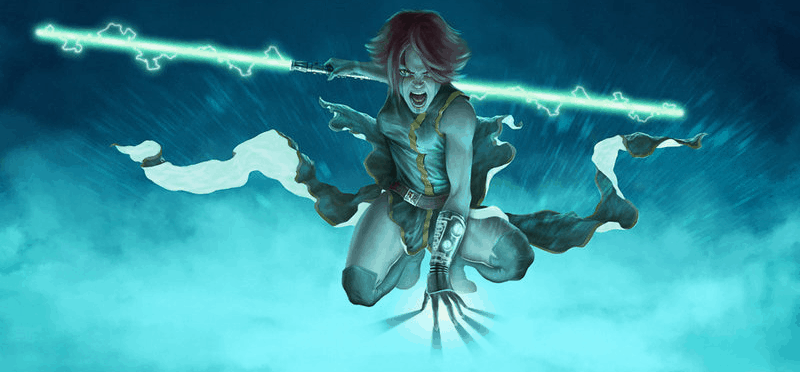
\includegraphics[width=\paperwidth]{_img/cover-bg.png}}
	\begin{tikzpicture}[overlay]
		\node[minimum width=180pt,minimum height=180pt, rotate=30] at (15,11){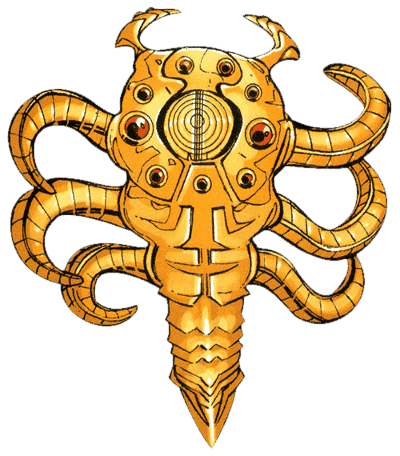
\includegraphics[width=180pt]{_img/dos-au-muur/talisman.png}};
	\end{tikzpicture}}
	\end{titlepage}

	\onecolumn
	\section{contexte de campagne}
	
	\begin{wrapfigure}{R}{180pt}
		\centering
		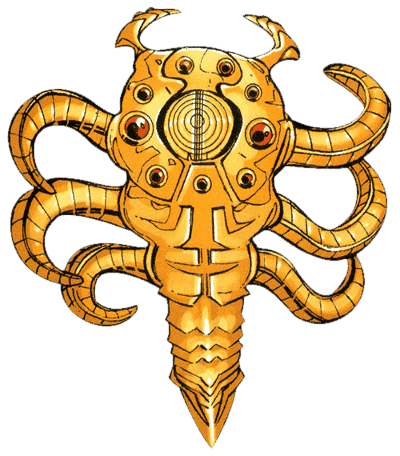
\includegraphics[width=180pt]{_img/dos-au-muur/talisman.png}
		\caption{\label{fig:talisman-de-muur}Talisman de Muur}
		\vspace{1\baselineskip}
		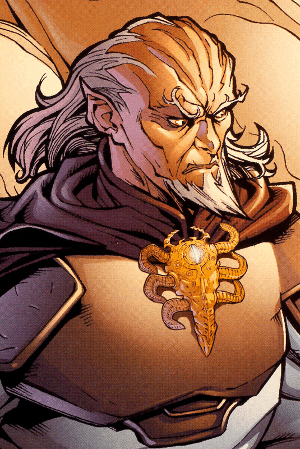
\includegraphics[width=180pt]{_img/dos-au-muur/karness-muur.png}
		\caption{\label{fig:karness-muur}Karness Muur}
	\end{wrapfigure}
	
	Cette campagne est écrite initialement pour \citetitle{jdrp-starwars} mais un scénar reste un scénar et il est jouable dans n’importe quel univers de Star Wars.

	L’idée était de faire une campagne d’introduction avec des personnages partant de rien. Les joueurs commencent Novice et n’ont pas besoin d’historique complexe et élaboré (bien que cela ne soit pas interdit bien sûr). De cette façon, les personnages devraient être assez vite fait. Et elle est adaptable aussi bien avec des joueurs orienté Alliance Rebelle que Empire. Dans les deux cas, l’objectif sera le même mais les dessains changeront.

	La campagne se déroule dans les premières années de l’avènement de l’Empire, au MJ de voir s’il veut préciser.

	La trame de la campagne se base sur un très ancien artéfact Sith, le \citetitle{talisman-de-muur}. Un artéfact créé par Karness Muur, un Sith se servant de la Force pour prolonger sa vie. L’artéfact contient l’âme de Muur, celui qui le porte est possédé par Karness et peut contrôler les Rakghoules.


	On trouve beaucoup d’informations sur cet artéfact sur HoloNet et je me suis grandement inspiré de ces informations pour cette campagne en faisant vivre à mes héros les aventures des divers individus qui ont croisé le Talisman\ldots

	\twocolumn

	\section{Sauvetage du Pelican}

Voici un scénario d'introduction pour la campagne \textbf{Dos au Muur}. Cette campagne est écrite initialement pour \citetitle{jdrp-starwars} mais un scénar reste un scénar et il est jouable dans n'importe quel univers de Star Wars.

Il est adaptable aussi bien avec des joueurs orienté Alliance Rebelle que Empire. Dans les deux cas, l'objectif sera le même mais les dessains changeront.

La campagne est faite pour des joueurs débutant, partant du rang Novice.

\vspace{2\baselineskip}
\begin{flushright}
	\emph{Pelican (IA-1701)}
\end{flushright}

\vspace{-4\baselineskip}

\hspace{-0.4\columnsep}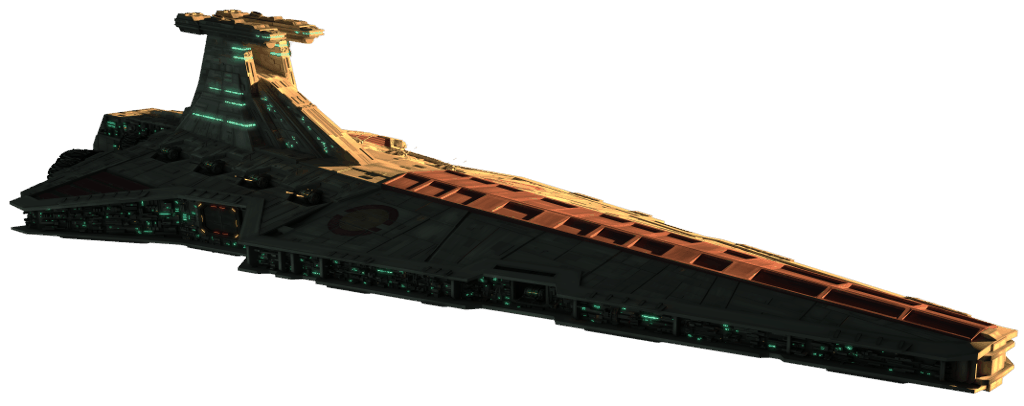
\includegraphics[width=\textwidth]{_img/dos-au-muur/venator.png}
\vspace{-7\baselineskip}

\subsection{La rencontre}
Nos héros ne se connaisent pas encore. Ils ont répondu à un contract proposé par \emph{Industrial Automaton} pour une mission de récupération.

Ils ont rendez-vous sur l'avant poste commercial de l'anneau de Kafrene au Starlord Café. \'A leur arrivé, ils sont conviés dans une arrière salle ou les attend Vyna Anen un Sluissi, le représentant de IA. En plus du groupe de nos héros, deux autres personnes ont répondu au contract, un Abyssin et un Rodien.

\begin{quote}
	Messieurs bonjour, je représente Indrustrial Automaton.
	Comme vous avez peu le voir sur le contract auquel vous avez répondu, nous cherchons a rassembler une équipe pour récupérer l'un de nos prototype de droïde Type R perdu sur Croiseur dont nous n'avons plus de nouvelle.
	Le \textbf{Pelican IA-1701} n'a plus donné signe de vie depuis 10h et 33mn maintenant. Il avait a son bord le seul prototype de notre dernier Type R. Il est vital pour nous de récupérer ce prototype intact.

	Si vous acceptez la mission, une navette droïde vous conduira directement à la dernière position connu du Pelican. Cette mission doit resté confidentielle, nous ne tenons pas à ce que le public sache qu'Industrial Automaton perde ses vaisseau !
	En cas de succés la somme convenue sera virée directement sur vos comptes respectif. Dans le cas contraire vous serez mort ou en passe de l'être.

	Il y a t'il des questions ?

	\ldots

	Bien, la navette décollera de l'astroport, quai N°5 dans une heure, elle n'attendra personne.
\end{quote}

Voilà qui donne le ton et la direction du scénario. Les héros disposent donc d'une heure, s'ils le souhaitent pour faire quelques amplettes puis direction la navette.

\subsection{Pelican Bay}
\'A la sortie d'hyperespace, les héros trouvent croiseur de classe Venator en bon état mais à la dérive. La navette tente une procédure d'appomtage mais le système de guidage ne semble pas fonctionner, le droïde aux commande de la navette ne cesse de répéter 

\begin{flushright}
		Erreur trop bas tros bas !\\
		Erreur trop bas tros bas !\\
		Erreur trop bas tros bas !\\
		Erreur trop bas tros bas !\\
		\ldots
\end{flushright}

\vspace{5\baselineskip}
Et la navette s'échoue lamentablement dans le hangard. Comme de par hasard, et pour bien appuyer sur le gravité de la situation, l'Abyssin et le Rodien sont mort pendant le crash et le droïde pilote est dans un sale état. Il ne pourra donner aucune information.

Une fois à bord du Pelican, une alarme est en cours et une voie pré-enregistré se fait entendre à intervale régulier :

\begin{quote}
	Alerte trajectoire, le vaisseau se dirige actuellement vers une étoile, point de non retour dans 2h53mn ! 
	Voyez modifier la trajactoire du vaisseau !\\ 
	\ldots
\end{quote}

\'A l'intérieur du vaisseau c'est la désolation, des cadavres partout, du sang sur les murs, des traces de griffures sur les murs. L'éclairage est partiellement en panne les neons scintilles, des débrits entravent la marche des héros. Leur champ de vision est réduit à cause des conditions à bord. Malgrés tout ça, les systèmes de survit et la gravité artificielle fonctionne.\\

Le bruit du crash de la navette a attiré la population locale, a savoir les Rakghouls~\ref{sec:rakghoul} (p. \pageref{sec:rakghoul}). Lancer 1d4 pour savoir combien se pointent. Si vous n'avez que 2 ou trois héros sous la main, ajustez avec 1d4-1.

\noindent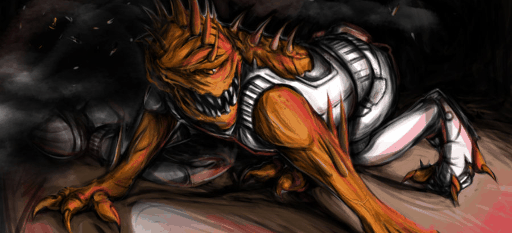
\includegraphics[width=\linewidth]{_img/dos-au-muur/rakghoul.png}

Le but des héros devrait maintenant être double, trouver le fameux prototype mais aussi trouver un moyen de sauver leur peau. 

\subsection{Exploration}
\emph{Numéroté les pièces de votre vaisseau et lancez un dé pour savoir dans qu'elle pièce se trouve le droïde.}\\

Une fois la première vague de Rakghouls balayé, nos héros se retrouvent dans le hangard, la porte de se dernier est ouverte.

Un jet de Recherche (-2 pour l'obscurité) réussi permet de trouver un kit de survie avec un Medipack, une lampe torche et des ratio de survie.

Pas loin de la porte du hangard se trouve un terminal dont l'écran clignote en rouge au rythme de l'alarme. Les héros peuvent tenter des jet de Piratage pour les actions suivantes :
\begin{rebelist}
	\item Stopper l'alarme. 
	\item Obtenir un plan du vaisseau. En cas de succés, le plan s'affiche mais le terminal rend l'âme au bout de quelques secondes et le plan s'efface. En cas de relance le plan reste affiché et le terminal est utilisable.
	\item  Obtenir l'inventaire des navettes présentent dans le hangard du vaisseau. Un succès leur apprend qu'il y en a une dans le hangard du niveau inférieur. Une Relance leur apprend que la navette est dans le hangard 4-2.
\end{rebelist}
Dans tout les cas, un échec critique fait disjoncter le terminal définitivement.

Les héros avancent donc dans les couloirs du Pelican à la recherche du droïde et d'un moyen de dévier le vaisseau. Faites faire un jet de Discrétion de temps à autre. En cas d'échec, 2 Rakghouls se pointent (plus si vous voyez que vos héros s'en tire trop facilement).

Au fur et mesure que les aventuriers avancent, utilisez les tuiles pour découvrir la carte du vaisseau.

\subsubsection{Le Droïde}
Quand les héros arrivent dans la salle où se trouve le droïde, ce dernier les menace avec un arc électrique, rien de bien méchant mais les héros doivent le rassurer et Négocier (jet de Persuasion) avec le droïde ou le Pirater (jet de Piratage opposé à l'Intellect). Dans les deux cas, avec un succés, le droïde les aide, leur montre le journal de bord. Avec un relance, le droïde devient un accolyte du héros qui a fait l'action. En cas d'échec le droïde refuse de les aider il se désactive. En cas d'échec critique, le droïde s'en prend à eux.

Si le droïde se désactive, un héros peut tenter de lui retirer la mémoire pour récupérer les infos avec un jet de Réparation. 

\subsubsection{Les Quartiers}
Il s'agit des quartiers de l'équipage. Pas grand chose à y trouver, des vètements, des effets personnels. On y trouve des terminaux qui peuvent être Piraté pour le plan du vaisseau ou pour d'auters information. Avec un succès, ils se connectent et ont accès au contenu du PC. La carte s'ils la cherche, sinon rien de fou, des photos, des vidéos et des films X.

\subsubsection{Les Laboratoires}
La porte du premier labo que les héros visitent est verrouillé. un jet de Piratage la déverrouille. Si le droïde est avec eux et les aide, il peut ouvrir toutes les portes. Les aventuriers trouvent dans ce labo le corps corps du rakghoul et un terminal. Un Piratage (malus -2, c'est un terminal sécurisé) leur donne les informations sur l'autopsie (cf. Le journal de bord~\ref{sec:pelican-jdb} p. \pageref{sec:pelican-jdb}), pas plus sur les circonstances.

Dans les autres labo, un jet de recherche donne un Medipac supplémentaire.

\subsubsection{L'Armurerie}
Dans cette pièce se trouve des cellules énergétiques pour les armes et des armes mais enfermées dans des casiers. Un coup de blaster ouvre les casiers. On trouve alors 5x Blaster Semi-Automatique (2d8 (3)) et 1x Lance Grenade (2d10 (1)), 5x Grenade (3d6).


\subsubsection{Le Pont}
La pièce est verrouillée et ne peut être ouverte avec un Piratage. Seul le droïde peut l'ouvrir. Si le droïde disparait ou s'éteind, la salle s'ouvre. Les héros en entrant dans la pièce trouvent le corp sdécomposé du commandant. En recherchant dans les poches du commandant, ils trouvent un document marqué "Protocole d'Urgence" expliquand la marche à suivre en cas de problème (cf. Le journal de bord~\ref{sec:pelican-jdb} p. \pageref{sec:pelican-jdb}). Le papier contient aussi les les codes d'accès au terminal.

Les héros peuvent donc accéder au journal de bord~\ref{sec:pelican-jdb} p. \pageref{sec:pelican-jdb}) avec toutes les infos. Si cela n'est déjà connu, ils savent qu'un vaisseau en état les attends dans le hangard 4-2 et il est possible d'en ouvrir la porte depuis ce terminal. S'ils sont malin, il est possible de voir ce qui les attends dans le hangard via des caméra de surveillance. Il peuvent aussi déclencher l'autodestruction.

\begin{paperbox}{Objectifs}
Les joueurs doivent d'une manière ou d'une autre apprendre l'histoire des rakghoul et du Talisman. Donc soit par le droïde, soit par le pont. Une fois qu'une des deux étapes est faite, l'autre n'est pas obligatoire. Donc peu importe qu'il déglinguent le droïde.
\end{paperbox}

\subsection{Le Hangard 4-2}

\noindent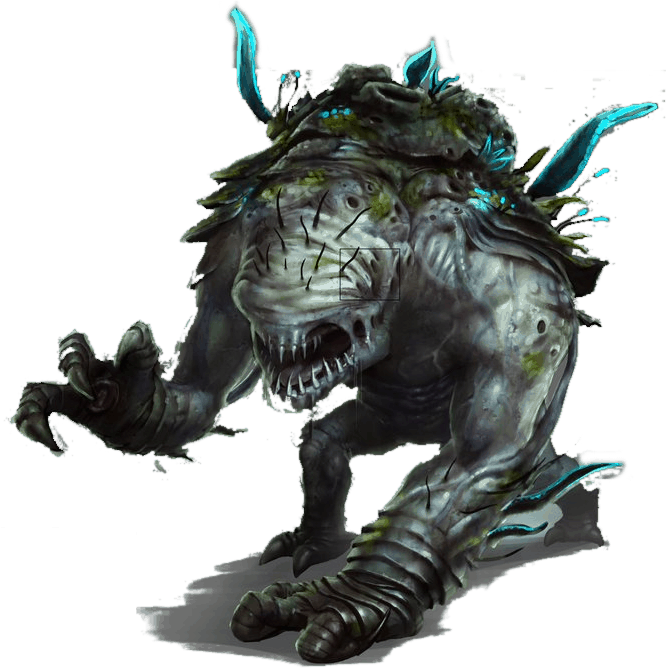
\includegraphics[width=\linewidth]{_img/dos-au-muur/rakghoul-amblyope.png}

Situé au pont inférieur, deuxième hangard. C'est l'étape final et le boss de fin du scénario.

Le droïde ou un passage au poste de commande déverrouille la porte du handard. \'A l'intérieur c'est une autre histoire, une créature de 2m de haut manifestement un rakghoul aux stéroïdes, un rakghoul Amblyope~\ref{sec:rakghoul-amblyope} p. \pageref{sec:rakghoul-amblyope}).

Selon vos héros et leur état, accompagnez le joker avec quelques rakghouls en extra. Les héros avec Sens de Force ressentent une forte présence du coté obscur autour de la créature.\\

Une fois le combat terminé, il ne leur reste plus qu'a prendre le vaisseau (Cargo léger YZ-775). Ouf, les clefs sont sur le contact. L'armement du vaisseau est endommagé et ne fonctionne pas mais le reste est intact.

\subsection{To be continue\ldots}
Une fois en vol, vos héros reçoivent une communication d'origine inconnue, le visage d'une femme apparait

\begin{quote}
	Tinon \emph{(prononcer Taïnon)} c'est toi ? Que se passe t'il ou va tu ?
\end{quote}

Rideau, suite au prochain épisode\ldots

%http://www.starwars-holonet.com/encyclopedie/technologie-talisman-muur.html

\clearpage
\section{Pelican (iA-1701)}

Quelques information sur le Pelican. C'est un croiseur de classe Venator. 1 137 m de long, 7400 hommes d'équipage, capable d'hyperpropulsion.

Le Pelican appartien à Industrial Automaton qui s'en sert comme vaisseau scientifique ultra-sécurisé. Ils y hébergent des projets top secret et au limite de la loi.

\subsection{Journal de bord}
\label{sec:pelican-jdb}
En relation étroite avec l'Empire, Industrial Automation envoie le Pelican à la recherche d'un ancien artéfact Sith, le Talisman de Muur. Le Pelican à fini par trouver une trace du Talisman sur Taris mais le Talisman n'y est plus, par contre en fouillant les bas fonds de la planète, l'équipe de chercheur trouve un temple Sith. Mais ce dernier est infesté de Rakghouls. L'unité de sécurité qui accompagne les chercheurs parvient à se débarrasser des quelques créatures mais plusieurs hommes sont blessés pendant le combat. Dans les ruines du temple le Talisman n'est plus là mais des indices tendent à penser qu'il a été transporté il y a très longtemps vers \emph{Jebble} (Planète glacière dans la bordure extérieure). Les scientifiques décident de ramener l'un des corps de Rakghoul à bord du Pelican pour l'étudier.

En chemin vers Jebble les scientifiques étudient le corps du Rakghoul et apprennent qu'il s'agit d'une maladie artificielle créé il y a des millénaire par Karness Muur. La maladie se transmet par griffure ou morçure. Cette maladie est étroitement liée à la Force et il semble que les personnes sensibles à la force ne puissent être contaminées. Cependant le Rakghoul étudié a l'air d'être contaminé par une forme très basique du virus, certainement une exposition prolongé à l'artéfact.

Après une semaine de voyage, les problèmes ont commencés. Les soldats blaissés lors de la rixe contre les Rakghouls sur Taris commencent à se transformer en Rakghouls à leur tour et s'en prennent au membre de l'équipage. C'est une boucherie sans nom. Voyant ça, le commandant du Pelican enregistre le journal de bord sur un droïde Type R et tente de bloquer le cap du vaisseau sur l'étoile la plus proche mais la propulsion est endommagé et bien que la cap du vaisseau soit bloqué, ce dernier se contante de dériver.

\subsection{Industrial Automaton}
N'ayant plus de nouvelle du Pelican depuis son départ de Taris, IA part à sa recherche. Ils le retrouve et envoient une équipe mais là encore, plus aucune nouvelles. C'est alors qu'IA décide d'envoyer des mercenaires. Si le commandant à respecté le protocole, il suffira que les mercenaires ramène le droïde\ldots

\subsection{Plan du vaisseau}
\noindent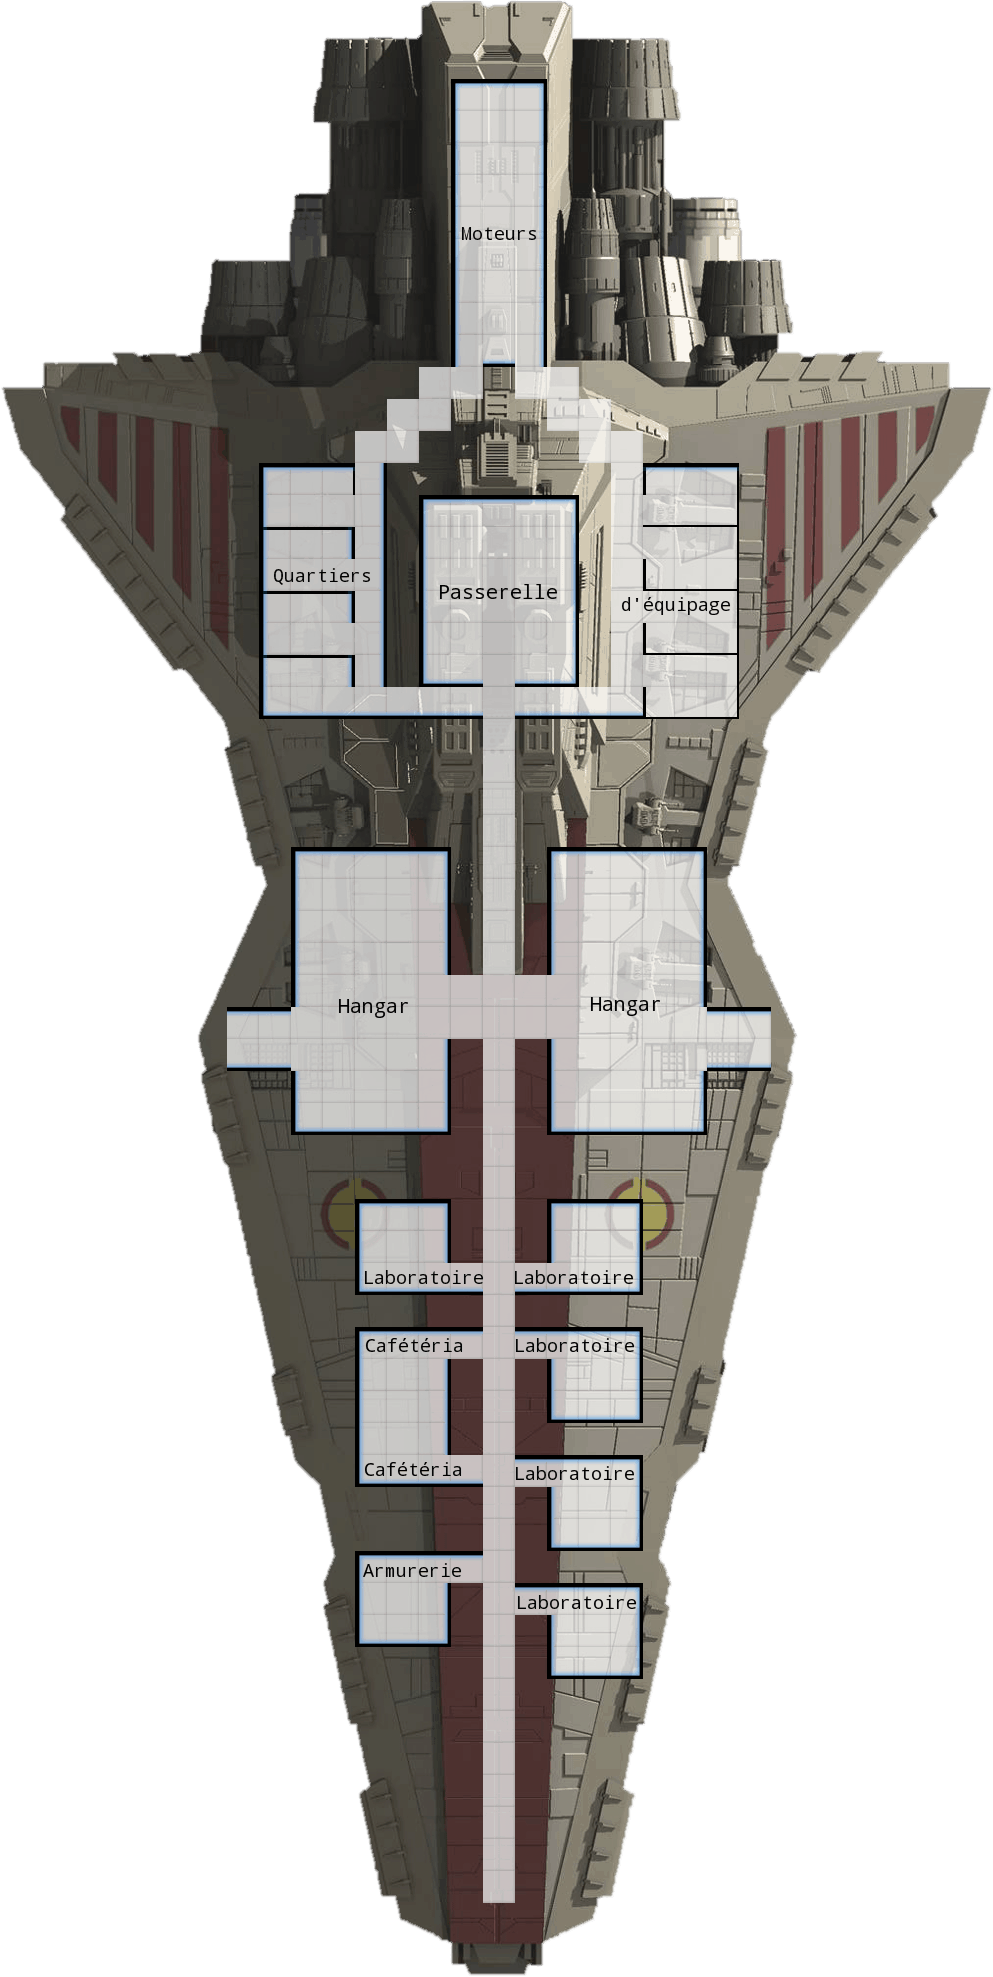
\includegraphics[width=\linewidth]{_img/dos-au-muur/venator-plan.png}

Ce n'est qu'une proposition, le plan peut changer à volonté. En annexe, vous trouverez des cases permettant de faire découvrire le vaisseau petit à petit aux héros.

\clearpage
\section{Bestiaire}

\subsection{Rakghoul}
\label{sec:rakghoul}
\noindent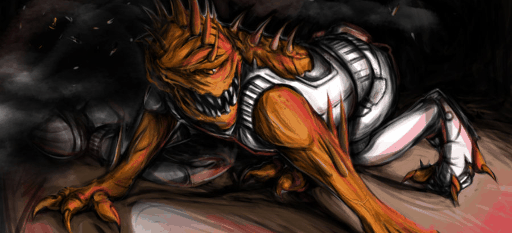
\includegraphics[width=\linewidth]{_img/dos-au-muur/rakghoul.png}

\subsubsection{Traits}

\begin{itemtable}[ c c c c c ]
    \textbf{Agi} & \textbf{Int} & \textbf{\^Ame} & \textbf{For} & \textbf{Vig} \\
    d8			 & d6			& d6			 & d8			& d8
\end{itemtable}
\begin{itemtable}[ l X ]
	\textbf{Allure} 	 & 6 \\
	~   				 & Vision Nocturne \\
	~   				 & Marche sur les murs \\
	\textbf{Compétences} & Combat d8, Discrétion d6
\end{itemtable}

\subsubsection{Défense}
\begin{itemtable}[ c c ]
	\textbf{Parade} 	& \textbf{Résistance} \\
	6					& 6 
\end{itemtable}

\subsubsection{Attaque}
\begin{itemtable}[ X c c ]
	~ 		& \textbf{Combat} 	& \textbf{Dégats} \\
	Griffes	& d8 				& 1d6 
\end{itemtable}

\newpage
\subsubsection{Background}
Les Rakghouls sont une espèce issue d'une maladie créée par le seigneur Sith Karness Muur. Les individus ateint par cette maladie deviennent des monstres incapable de penser par eux même. Karness peut les contrôller grâce à son talisman (Le Talisman de Muur).

La maladie se transmet par une griffure ou un morsure mais cela ne fonctionne pas avec les êtres sensibles à la Force. Karness a créé se virus à partir du coté Obscur de la Force ce qui explique une forte présence obscure près de ces monstres.

Karness a créé plusieurs versions du virus car les premiers Rakghouls ne répondaient pas bien au contrôle de Karness. Les nouveaux sont plus réceptif et plus fort.

Quand le Talisman de Muur a été perdu dans les bas fonds de Taris, on a peu constaté que les créatures, suite à une exposition prologé au Talisman finissaient par se transformer en Rakghouls. Mais les Rakghouls transformé de cette façon sont bestiaux, stupide et sans âme. Ils attaquent tout ce qui bouge. Ces créatures ne fonctionne qu'à l'instinct.

\clearpage
\subsection{Rakghoul Amblyope}
\label{sec:rakghoul-amblyope}
\noindent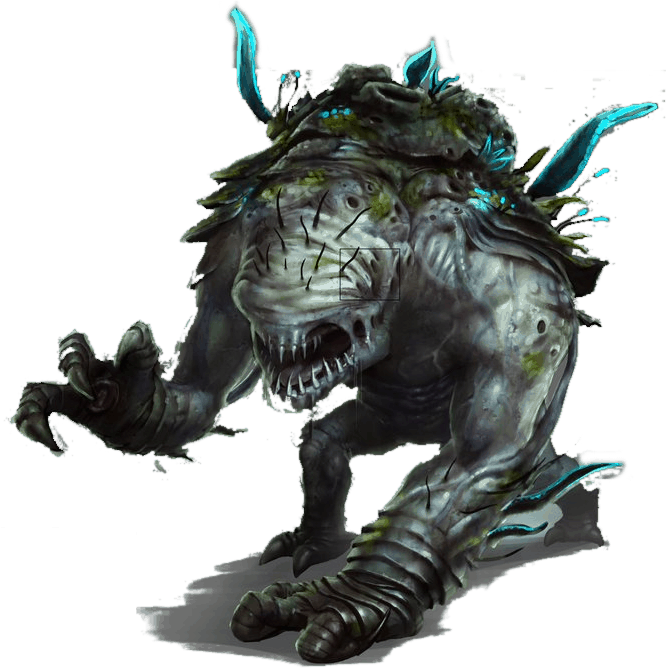
\includegraphics[width=\linewidth]{_img/dos-au-muur/rakghoul-amblyope.png}

\subsubsection{Traits}

\begin{itemtable}[ c c c c c ]
    \textbf{Agi} & \textbf{Int} & \textbf{\^Ame} & \textbf{For} & \textbf{Vig} \\
    d4			 & d6			& d6			 & d12+2		& d10
\end{itemtable}
\begin{itemtable}[ l X ]
	\textbf{Allure} 	 & 5 \\
	\textbf{Taille} 	 & +5 \\
	~   				 & Vision de Force \\
	~					 & \'Enorme (+2 pour les jets d'attaque adverses)\\
	\textbf{Compétences} & Combat d10
\end{itemtable}

\subsubsection{Défense}
\begin{itemtable}[ c c ]
	\textbf{Parade} 	& \textbf{Résistance} \\
	5					& 12 
\end{itemtable}

\subsubsection{Attaque}
\begin{itemtable}[ X c c ]
	~ 			& \textbf{Combat} 	& \textbf{Dégats} \\
	Mains nues	& d10 				& d12+2 
\end{itemtable}

\newpage
\subsubsection{Background}
Version stéroïdé des Rakghouls standard, Amblyope est notre petit boss de niveau.

Quand les Rakghouls sont livrés à eux mêmes et qu'il laisse libre court à leurs plus bas instincts, il arrive qu'un Rakghoul plus fort que les autres s'en prenne à ces petits camarades et les dévore sans scrupule. Cette afflut de Force Obscure peut le faire muter et le Rakghoul devient une espèce de gros monstre de 3m de haut, complètement aveugle mais attiré par les émanation de Force, il attaque machinalement les adversaires les plus sensible à la Force. 

\clearpage
\subsection{Vyna Anen}
\noindent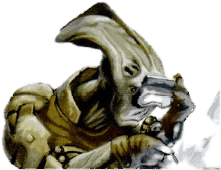
\includegraphics[width=\linewidth]{_img/dos-au-muur/vyna-anen.png}

\subsubsection{Traits}

\begin{itemtable}[ c c c c c ]
    \textbf{Agi} & \textbf{Int} & \textbf{\^Ame} & \textbf{For} & \textbf{Vig} \\
    d6			 & d10			& d6			 & d4			& d6
\end{itemtable}
\begin{itemtable}[ l X ]
	\textbf{Allure} 	 & 6 \\
	\textbf{Compétences} & Intimidation d6, Persuasion d12, Réseaux d6
\end{itemtable}

\subsubsection{Défense}
\begin{itemtable}[ c c ]
	\textbf{Parade} 	& \textbf{Résistance} \\
	2					& 5 
\end{itemtable}

\newpage
\subsubsection{Background}
Vyna Anen est l'un des agent de liaison entre Industrial Automaton et l'Empire. Officiellement employé par IA comme secrétaire au service des "Projets Spéciaux". 

Vyna est un homme pragmatique qui fait ce que l'Empire lui demande sans poser de question, sans scrupule ni état d'âme. C'est une fin négociateur entièrement voué à l'Empire.\\

\noindent
\includegraphics[width=\linewidth]{_img/dos-au-muur/industrial-automaton.png}

\subsection{Droïde R4 [Joker]}


	\section{Les bas fonds de Taris}

C'est partie pour le deuxième volet de la campagne. C'est un épisode qui peut, selon les choix des héros, être assez long. L'épisode précédent était d'environ deux heures, cet épisode peut durer jusqu'à 4 heures selon les direction prises. Il peut aussi être beacoup plus court si les héros empruntent tous les raccourcis. C'est a vous de doser les ennemis et les choix pour adapter le temps de jeu à ce que vous souhaitez.

\subsection{Prologue}
Nos héros se retrouvent donc dans un Cargo léger YZ-775 sans canons fonctionnel et un message entrant d’une inconnue qui demande à parler à Tinon.

Ils ont aussi apris qu’Industrial Automaton sous couvert d’expérimentations de son nouveau modèle, fait des recherches sur un très ancien artefact Sith en provenance de \textbf{Taris}. De plus, s’ils ont réussi à récupérer le droïde, Vyna Anen les attend sur l’avant-poste commercial de \textbf{l’anneau de Kafrene} au Starlord Café. Enfin, ils savent aussi que le vaisseau se dirigeait vers \textbf{Gaulus} pour rejoindre un laboratoire de l’empire où il devait finir des recherches sur l’artéfact.

Plusieurs directions s’offrent alors à nos héros.

\subsection{Les bons, les brutes ou les truants}
\begin{quotebox}
    Tinon \emph{(prononcer Taïnon)} c’est toi ? Que se passe t’il ou va tu ?
\end{quotebox}
Le visage d’une jeune femme apparait sur l’holocomm. Les héros ont le choix de répondre ou non.

Ce point de l’aventure est crutial pour nos héros car ils vont choisir (en connaissance de cause ou non) l’orientation de leurs personnages. En effet plusieurs cas de figures se présentent :

\begin{description}
    \item[\nameref{sec:les-rebels}] Répondre au message et suivre les consignes des Rebels (page~\pageref{sec:les-rebels}).
    \item[\nameref{sec:retour-du-droide}] Ramener le droïde à Vyna Anen (page~\pageref{sec:retour-du-droide}).
    \item[\nameref{sec:refus-d-obtemperer}] Partir pour Taris directement (page~\pageref{sec:refus-d-obtemperer}).
    \item[\nameref{sec:l-empire}] Prendre la direction de Gaulus (page~\pageref{sec:l-empire}).
\end{description}

Tous ses choix amèneront, de toute façon, les héros sur Taris mais le chemin sera différent et par là même leur orientation aussi. Je vais tacher de décrire les choix possibles sachant que rien n’est écrit dans le marbre et vous pouvez très bien les forcer suivre une route en particulier. C'est un peu le jeu de piste, les choix s'entrecroisent alors faut suivre. Mais une fois de plus rien n'est définitif, les joueurs auront toujours des idées farfelues auquelles on a pas pensé mais je vais essayé de décrire les principales voies possibles, au MJ de diriger les joueurs vers une de ces voies.


\subsubsection{Retour du droïde} \label{sec:retour-du-droide}

Autre choix possible pour les héros, ces derniers, avident de crédits, veulent allez rendre le droïde et récupérer le solde promis pour leur mission. Il retournent donc sur l'avant-poste commercial dans \textbf{l'anneau de Kafrène} ou les attend \nameref{sec:vyna-anen}.

On laisse les héros discuter un peu et réclamer leur due, Vyna acquiesce avec le sourire, leur donne les crédits mais au moment de quitter la pièce, 4 ou 5 \textit{(doser en fonction du niveau de vos joueurs)} Stormtroopers leur barre la route. Attention, à moins que les héros est anticipé, le premier tour de combat sera pour dégainer.

\begin{quotebox}
    Vous pensiez réellement qu'avec tout ce que vous savez, nous allons vous laisser repartir tranquillement ?\\
    Commencez par me rendre les crédits.
\end{quotebox}

Les héros peuvent tenter de négocier avec Vyna, ce dernier acceptera de les laissé repartir vivant (mais sans crédit) à condition qu'ils retourne sur \nameref{sec:taris} et recupèrent les informations que les scientifiques de Industrial Automaton n'ont pas eu le temps de récupérer. Ils peuvent tenter un jet de Persuasion pour garder les crédits.\\

Si les héros entrent en combat, et qu'ils perdent, on ne les tue pas mais Vyna leur impose de retourner sur Taris et pas de négociation possible. S'ils gagnent, deux cas de figure possible :
\begin{rebelist}
    \item \textbf{Ils tuent Vyna} Un homme, Chiss, manifestement important en uniforme de l'empire entre dans la pièce en applaudissant. Pausément, il félicite les joueurs et   leur expliquent qu'il ont réussi le test avec brillo. Vyna était devenu génant pour l'empire et pour l'Odre. Si l'un des héros tente quoi que ce soit il se retrouve désarmé et collé au mur avant d'avoir eu le temps de comprendre. On déccroche sur \nameref{sec:l-empire}.

    \item \textbf{Ils laisse Vyna en vie} Une femme (celle qui est apparue sur le holocom du vaisseau) entre dans la pièce avec deux hommes. Les deux hommes emportent Vyna avec eux, en faisant comme s'il était ivre. Et la femme leur fait signe de la suivre vite, elle leur expliquera plus tard. Ils prennent le vaisseau et partent pour la cache des Rebels. On déccroche sur \nameref{sec:les-rebels} dans la version bien accueilli.
\end{rebelist}

Le \nameref{sec:nimbus} n'est réparé qu'à leur demande, le prix est de 40 000 \crg. Négociable (Persuasion) à 30 000, -10k si relance.


\subsubsection{Les rebels} \label{sec:les-rebels}

\begin{quotebox}
    Tinon \emph{(prononcer Taïnon)} c’est toi ? Que se passe t’il ou va tu ?
\end{quotebox}

Le visage d’une jeune femme apparait sur l’holocomm et les héros choisissent de répondre.

\begin{quotebox}
    Mais qui êtes vous et où et Tinon ?
\end{quotebox}
Les joueurs choisissent de raconter leur histoire, ou de mentir, à voir ce qu'ils préfèrent. Lindi leur demande de la rejoindre et leur donne les coordonnées d'une cache de la Rébellion. Si les joueurs ont menti, il sont accueilli avec suspicion, menacé et tout ce qui va avec, sinon ils sont accueillit normalement avec juste un peu de méfiance. \nameref{sec:lindi-dangon} les invite à la suivre et les interroge jusqu'à ce qu'ils disent la vérité (On part du principe que s'ils persistent à mentir, on bifurque vers l'option \nameref{sec:refus-d-obtemperer}).

Lindi leur explique alors que la résistance à eu vent des recherches mené par l'Industrial Automaton ainsi que des problèmes sur le Pelican. \textbf{Tinon Dystra} avait été envoyé pour tenté de s'infiltrer à bord du Pelican. Mais qu'il n'avait plus donné de nouvelles depuis son arrimage au vaisseau.

Un jet de \textbf{Perception} ou l'utilisation de \textbf{Sens de Force} fera apparaître les sentiments de Lindi envers Tinon et apprendra à nos héros que ces derniers étaient amants.\\

Une fois la discution terminé, Lindi demande de l'aide aux héros, qu'ils reprenne le travail de Tinon. La première piste à explorer étant \ldots \nameref{sec:taris}.

Le \nameref{sec:nimbus} est réparé gratuitement pendant que les héros discutent.


\subsubsection{Refus d’obtempérer} \label{sec:refus-d-obtemperer}

Les héros veulent se la jouer et décident de partir direct sur Taris. Mais ils ne savent même pas trop se qu'ils y cherche. L'hyper-espace est récalcitrant et ne veut pas fonctionner immédiatement. Le temps de regarder, un croiseur sort d'hyper-espace et les arraisonne sans poser de question. Des soldats de l'alliance (trop pour être combattu) forcent la cloison et entre dans le cargo, suivi par la femme vu précédemment sur l'holocomm.

\begin{quotebox}
    Où pensiez vous partir comme ça avec ce cargo ? \\
    \emph{se retournant vers les soldats}, jetez moi ça en cellule on les interrogera là bas.
\end{quotebox}

Les héros sont transporté jusqu'à une cache de la Rébellion et jeté en cellule. Au bout de quelques temps, la femme précédement rencontré vient les interroger. Ils ont le choix de répondre la vérité ou de mentir. S'ils répondent la vérité, on déccroche sur l'option correspondante dans \nameref{sec:les-rebels}. Sinon ils sont laissé en cellule \ldots

Mais dans la nuit, un mystérieux inconnu s'approche de la cellule sans bruit

\begin{quotebox}
    Je suis envoyé par Vyna Anen, si vous voulez vivre, venez avec moi et ne faites pas un bruit.
\end{quotebox}

L'inconnu ouvre leur cellule et les emmène au Cargo. Sur le chemin, leur demander des jets de \textbf{Discrétion}. En cas d'échec deux soldats débarquent. Dans le hangar où se trouve le Cargo, 4 soldats montent la garde. Soient les héros passent en force et débute un combat puis vont ouvrir les portes du hangar. Soit ils la jou furtif, se glissent dans le vaisseau et tire sur les portes pour sortir du hangar. Ou n'importe quoi d'autre qui leur permet de sortir. Une fois dehors l'inconnu leur transmet des coordonnées. Ils n'ont pas le choix, s'ils font mine de résister, l'inconnu sort une arme et les tiens en joue. Eux n'ont pas d'arme ils sortent de cellule. On déccroche ensuite sur \nameref{sec:l-empire}.



\subsubsection{L’empire} \label{sec:l-empire}
Enfin, dernière alternative les héros peuvent vouloir partir pour \textbf{Gaulus} la planète vers laquelle se dirigeait le vaisseau. 

A l'approche de la planète, le cargo est arraisonné par un croiseur de l'empire. Les héros sont invité à sortir et une dizaine de Stormtroper les attendent. Ils sont escroté jusque dans un bureau où les attendant \nameref{sec:vyna-anen} et un Chiss en uniforme de gradé de l'empire. C'est ce dernier qui prend la parole.

\begin{quotebox}
    Messieurs (mes dames) nous vous attendions. Asseyez vous je vous pris. \\
    Alors comment s'est passé cette mission, je vois que tout le monde n'est pas revenu \emph{(sourire aux lèvres)}. 
\end{quotebox}

Le droïde est emmené par deux gardes. Puis le Chiss se présente.

\begin{quotebox}
    Je me présente, je m'appelle \nameref{sec:garan-keggle}, j'ai suivi la mission de loin et je tiens à vous féliciter, vous vous en êtes sorti plutôt bien. Je pensais pas que vous viendriez à bout de l'Amblyope mais j'avoue que le combat était intéressant. Au vue de vos qualités respective, je souhaiterais que vous partiez pour \nameref{sec:taris} afin de finir la travail \emph{(il jette un regard froid sur Vyna qui en même pas large et baisse les yeux)} nous avons besoin de plus d'information sur la position de l'artéfact.
\end{quotebox}

Si les héros se hasard à demander un prime, on leur répond que l'empire saura les récompenser sans plus de détail. S'il sont récalcitrant on leur explique que c'est pas une proposition que l'on vient de leur faire.


\subsection{Taris} \label{sec:taris}
\noindent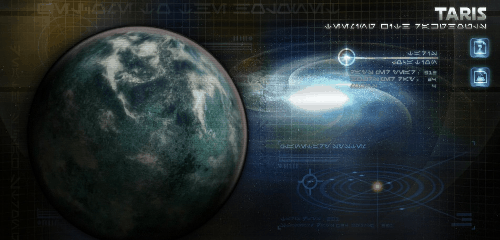
\includegraphics[width=\linewidth]{_img/dos-au-muur/taris.png}
Taris est une planète urbaine, très polluée, de la Bordure Extérieure. Divisée en trois grandes parties en fonction des étages, la Ville Haute, la ville basse et les "bas fonds", elle abritait autrefois une population gigantesque. Grand pôle économique dans la galaxie, notamment grâce à l’implantation des industries Lhosan, elle joignit la République Galactique peu avant les Guerres Mandaloriennes. Mais après la passage de Dark Malak plus de 4000 ans auparavant la planète à du mal à reprendre vie. Les "bas fonds", qui abritaient toutes sorte de hors la loi et de rebus de la société, est la partie de Taris qui s'en est le mieux sortie et c'est pourquoi les ruines marécageuses de Taris sont très dangeureuses. La république a depuis implanté un spaciaux port et une base militaire sur la planète dans l'espoir de la recoloniser mais le processus s'avère lent et compliqué.

Normalement une fois au spacioport, vos héros ne savent pas où aller. Plusieurs choix s'offre à vous pour les orienter. Est de leur placer un bar bien en évidence sur leur chemin. A l'intérieur ils pourront trouver des informations et peut être même un guide.

Normalement, ils vont se diriger vers le barman. Au pire, c'est le barman qui vient à eux pour leur demander ce qu'ils veulent boire. Ce dernier, un Besalisk, leur explique que l'endroit où ils souhaite se rendre (les ruines de l'ancien temple Sith) se trouve dans un zone interdite, au coeur de la zone de quarantaine \nameref{sec:rakghoul}. Il n'est pas possible de s'y rendre.

Mais un client du bar les accoste et leur dit que moyennant 20 000 \crg il les conduira où ils le souhaite. Un jet de Persuasion (opposé à la Persuasion de l’inconnu 5) fera descendre la somme à 15 000 \crg.

\begin{paperbox}{Quête annexe (optionnel)}
    Il est possible d'intégrer une petite quête annexe ici histoire de varier les plaisirs. S'ils la réussisse on pourra distribuer +1 XP supplémentaire.

    L'inconnu propose à vos héros de les conduire gratuitement aux ruines s'ils l'aide. Selon l'orientation des joueurs à ce moment, soit:
    \begin{description}
        \item [obscur] Ils aident un contrebandier à Kidnapper une jeune Twi'lek répéré dans un camp de réfigié pas loin.
        \item [clair] Ils aident un père à délivrer sa fille Twi'lek des mains de contrebandiers.
    \end{description}

    Le roleplay est un peu différent selon la situation mais la quête se déroule de la même façon. Les héros suivent l'inconnu qui s'est présenté entre temps (\nameref{sec:gil-harend}). Ce dernier les conduit au camp (de réfugiés ou de contrebandier). Un jet de Discretion réussi par tout le monde permet de s'approcher de la cible. Un jet de discrétion réussi par tous permet de s'extraire de camp sans encombre. Le joueur qui est chargé de transporté la cible à un malus de -2 à son deuxième jet de discrétion.

    Si une Discrétion est raté par l'un des joueurs, un combat commence. Vos héros se trouve confronté à H -1 contrebandiers/réfugiés (H est le nombre de joueurs que vous avez). Vos héros ont l'initiative sur le premier round. En face les ennemis ont les caractéristiques \nameref{sec:taris-contrebandier}.

    Attention, \nameref{sec:gil-harend} ne doit pas mourir sinon la quête est un échec et retour au bar. 
\end{paperbox}

\subsubsection{Les ruines de l'ancien temple Sith}
\noindent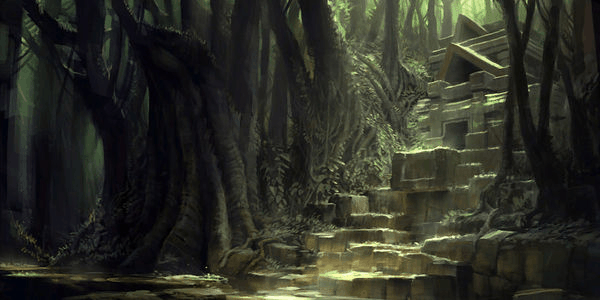
\includegraphics[width=\linewidth]{_img/dos-au-muur/taris-temple-sith.png}

Après plusieurs heures de marche dans les marécages de Taris, le groupe arriver devant les ruines de l'ancien Temple Sith. Le côté obscur de la Force émane du temple dans toutes les directions et l'atmosphère est pesante. D'ailleurs on entend absolument aucun bruit, comme si toute la faune avait déserté la zone. L'entrée est partiellement éboulée mais il reste une ouverture suffisante pour s'y faufiler.

Après être entré dans le temple les héros se retrouvent dans une immense salle, très haute de plafond. Deux rangées de statues de 10m de haut représentent d'anciens seigneurs Sith (Un jet de Connaissance (Sith) permet d'apprendre qu'il s'agit de Tulak Hord, Dakhan Shar, Naga Sadow, \ldots entre autres). Au fond de la salle une fresque murale est gravée sur un monolithe.

Chacun des murs de la pièce (en dehors de celui de l'entrée dans leur dos) possède deux ouvertures vers des pièces.

Devant le monolithe, les vestiges d'un campement de fortune (attention, c'est des vestiges de 3000 ans quand même, heureusement à l'époque on faisait les choses pour que ça dure ;-) ) recouvert de poussière. Une partie de ce campement semble pourtant avoir été remué récemment.

Naturellement, nos héros ne sont pas seul. 5 \nameref{sec:rakghoul} débarquent et encerclent les héros, s'en suit une phase de combat.
\\

Une fois les Rakghoul élliminés, les héros peuvent aller observer le monolithe et le campement.

<<insérer le dessin de la fresque>>

Un jet de \emph{Connaissance (Sith)} permet de comprendre la fresque. 

\begin{quotebox}
6 000 ans par le passé, un Jedi fut exilé pour ses penchants obscur et ses expériances interdites sur la vie. Son objectif était, en utilisant le coté obscur, de pouvoir plier la vie elle même à sa volonté et ainsi acquérir la vie éternelle. En étudiant l'alchimie du coté obscur il parvient à créer un Talisman renfermant son essence et sa volonté. Cet artéfact devait, entre autre, lui permettre de prendre posséssion du corp du porteur du Talisman mais aussi de contrôller les Rakghoul.

Ce Jedi Noir fut tué par un de ses rivaux et durant les décennies suivantes plusieurs Seigneurs Sith se déchirèrent entre eux afin de mettre la main sur ce Talisman. Enfin, l'artéfact et son porteur du moment finirent par être tué et enseveli dans ce temple au milieu des bas-fonds de Taris.
\end{quotebox}

S'ils ne font pas ce jet ou qu'ils le ratent, il ne peuvent que tenter d'interpréter la fresque. Après il leur est possible de faire des recherches sur cette fresque dans un temple Jedi ou une bibliothèque. En soit l'histoire n'a pas une grosse importance pour la suite, c'est un bonus pour eux.

Si l'un des héros possède vision de force et s'en sert, il pourra distinguer sur le monolithe un texte, le code des Sith écrit en lettres obscures
\begin{quotebox}
La paix est un mensonge, il n’y a que la passion. \\
Par la passion, j’ai la puissance. \\
Par la puissance, j’ai le pouvoir. \\
Par le pouvoir, j’ai la victoire. \\
Par la victoire, je brise mes chaînes. \\
La Force me libérera.
\end{quotebox}

Ensuite avec un jet de recherche sur le campement de fortune, ils trouvent un vieux datapad mais qui a besoin d'être chargé. Dommage, personne n'a de quoi l'alimenter sur lui (sauf si quelqu'un possède l'Atout \emph{Recycleur} et s'en sert). Il faudra trouver le matériel et faire un jet de \emph{Réparer} pour en tirer des informations.

Dans les autres pièces du temple si les héros éffectuent une recherche ils ne trouvent rien que des restes de Rakghoul et d'animaux à moitié dévorés.
A la sortie du temple, les héros sont attendu de pied ferme par 3 \nameref{sec:taris-contrebandier}s. C'est soit les contrebandiers à qui il s ont repris la jeune fille plus tôt qui viennent se rembourser. Soit les amis de \nameref{sec:gil-harend} qui a décidé de les doubler. Dans tout les cas, les contrebandiers veulent récupérer le datapad. Baston\ldots

Une fois débarrassé des contrebandiers, retour au spacioport où ils trouveront de quoi réparer le datapad et en tirer les informations qu'ils cherchent.

\subsection{\'Epilogue}
Le datapad appartenait à un certain \nameref{sec:pulsipher} qui en étudiant les archives du temple Jedi de Taris avait apris l'existence de l'artéfact. D'après les informations, Pulcipher a procédé à des excavations et a trouvé le Talisman de Muur. Mais il du plier bagage rapidement car 3 Jedis appartenant au Cercle de Veille de Taris arrivent pour récupérer le Talisman. Pulcipher quitte alors Taris à bord du Mar'eyce, qui prit la direction de \textbf{Jebble}

\subsection{Progression}
Toujours à titre indicatif:
\begin{rebelist}
    \item \textbf{1xp} Si ils sont passé par \nameref{sec:les-rebels} ou \nameref{sec:retour-du-droide}. Dans ces deux cas, les joueurs ont suent anticiper les évènements et n'ont pas cherché à tricher.
    \item \textbf{1xp} S'ils ont fait la quête annexe et l'ont réussit, que \nameref{sec:gil-harend} n'est pas mort.
    \item \textbf{1xp} S'ils ont peu traduire le monolithe ou le comprendre correctement.
    \item \textbf{1xp} S'ils se dirigent vers Jebble sans que personne ne soit mort.
\end{rebelist}

\newpage
\subsection{Nimbus} \label{sec:nimbus}
\vspace{-4\baselineskip}
\begin{figure}[h!]
    \centering
    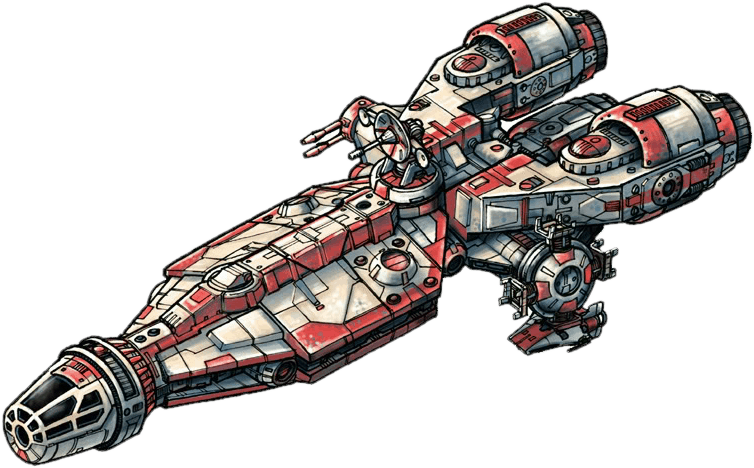
\includegraphics[width=\linewidth]{_img/dos-au-muur/nimbus.png}
    \caption{Cargo léger YZ-775}
\end{figure}

Le \textbf{Nimbus} est un cargo léger type YZ-775 modifié par l'alliance rebelle. 52m de long, 8 membres d'équipage, 12 passagers, 400 tonnes da charge utile. Coté armement il dispose de 1 canon turbolaser double, 2 canons-laser doubles, 2 lance-torpilles à proton.

Il appartient initialement à \nameref{tinon-dystra} qui s'en est servi pour infilter le \nameref{sec:pelican} lors d'une mission pour l'alliance. Malheureusement, il ne s'en est pas tiré et le Nimbus est resté à quaie sur le Pelican. D'où il a servi de nacelle de secour aux héros.

	\section{Laboratoire de Pulsipher}

\subsection{Jebble}
\noindent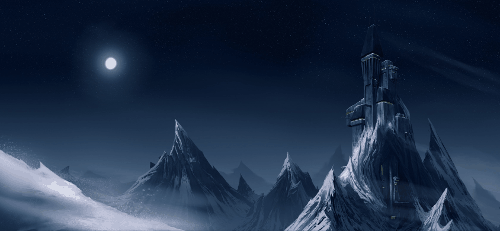
\includegraphics[width=\linewidth]{_img/dos-au-muur/jebble.png}
\'A l'extrémité de la bordure extérieure, complètement gelée à l’image de Hoth, Jebble constituait autrefois le dernier rempart de défence de la République contre les Mandaloriens. Jebble a été le théatre des évènements consernant le Talisman de Muur, Céleste Morne et \nameref{sec:pulsipher}. C’est durant ces évènement que la planète a été bombardé entièrement par la flotte de Cassus Fett afin d’éviter la contagion des Rakghouls. Ce bombardement a fait fondre les glaces de Jebble et les installation de Pulsipher ont coulé dans les eaux bouillonnates qui ont regelé par dessus.

Il y a plus de 1~000~ans des mineurs qui cherchaient a exploiter les ressources de la planète, sont tombé sur les installation de Pulsipher, y ont trouvé l'oubliette de Dreya qu'ils ont vendu en tant que « Boite de Jebble ».

Depuis la planète Jebble a sombré dans le déintéret le plus complet pour le reste de la galaxie.

\subsection{Astroport de Kriloo City}



%   L'épisode suivant se passe sur Jebble dans le labo du professeur Pulcipher. Où l'on apprend ce qu'il s'est passé pendant le voyage de retour. On trouve aussi des information sur l'oubliette de Dreypa et l'on a des piste sur l'endroit où elle se trouve. On entend notement parler de Céleste Morne.
%   Ici une idée est qu'au moment de quitté la planète pour l'étape suivante, les héros se retrouvent pris au piège par des troupes de l'empire qui on pris leur vaisseau en otage. Histoire de varier l'aventure. On peut même se mettre une petite baston spaciale.
%   Il faudra ensuite forcer les héros à retourner à leur QG (alliance rebelle ou empire) pour réparation et pour compte rendu.

%   Dans l'épisode suivant, le rebelles apprennent qu'on aurait vu le talisman sur une certaine lune de Jesaispasou et les soldats de l'empire apprenne qu'ils vont tendre un piège à l'alliance sur un lune de Jesaispasou.
%   Grossomerdo, Celeste se pointe et calme tout le monde, obligé de battre en retraite et de trouver un plan pour enfermer Celeste dans l'oubliette de Dreypa ou pour lui virer le Talisman avant d'enfermer ce dernier dans l'oubliette. Ou se trouve l'oubliette ? Quel est le plan ?
	\section{Personnages}
Les personnages avec un ‘ \textbf{*} ’ sont des Jokers, ils possèdent un fiche de perso jouable. 

Par ordre d’apparition :

\begin{figure}[h!]
    \centering
    
\includegraphics[width=\linewidth]{_img/dos-au-muur/industrial-automaton.png}
    \caption{Industrial Automaton}
\end{figure}

\newpage
\subsection{Vyna Anen} \label{sec:vyna-anen}
\noindent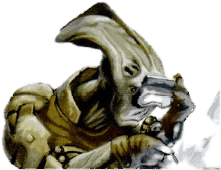
\includegraphics[width=\linewidth]{_img/dos-au-muur/vyna-anen.png}
\textbf{Race:} Sluissi

\subsubsection{Background}

Vyna Anen est l’un des agents de liaison entre Industrial Automaton et l’Empire. Officiellement employé par IA comme secrétaire au service des "Projets Spéciaux". 

Vyna est un homme pragmatique qui fait ce que l’Empire lui demande sans poser de questions, sans scrupules ni états d’âme. C’est un fin négociateur entièrement voué à l’Empire.

\subsubsection{Traits}

\begin{itemtable}[ c c c c c ]
    \textbf{Agi} & \textbf{Int} & \textbf{\^Ame} & \textbf{For} & \textbf{Vig} \\
    d6           & d10          & d6             & d4           & d6
\end{itemtable}
\begin{itemtable}[ l X ]
    \textbf{Allure}      & 6 \\
    \textbf{Compétences} & Intimidation d6, Persuasion d12, Réseaux d6
\end{itemtable}

\subsubsection{Défense}
\begin{itemtable}[ c c ]
    \textbf{Parade}     & \textbf{Résistance} \\
    2                   & 5 
\end{itemtable} 

\clearpage
\subsection{R4-3D*} \label{sec:r4-3d}

\clearpage
\subsection{Tinon Dystra} \label{sec:tinon-dystra}
\begin{figure}[h!]
    \centering
    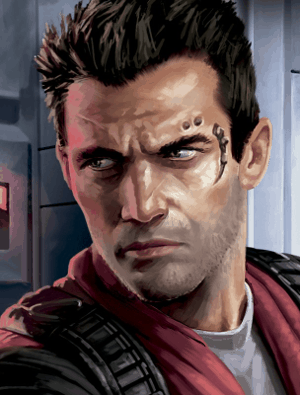
\includegraphics[height=250pt]{_img/dos-au-muur/tinon-dystra.png}
\end{figure}

\subsubsection{Background}
Ce personnage est mort quand débute le scénario mais il garde son importance car il est le lien entre les joueurs et l'alliance Rebelle.

Tinon est un membre de l'alliance rebelle envoyé en mission d'infiltration sur un vaisson de Industrial Automaton (Le \nameref{sec:pelican}) afin de découvrir ce qu'il s'y trame. Mais sa mission à mal tourné et il n'a plus donné aucune nouvelle. 

En fait il s'est infiltré à bord du Pelican alors que la maladie des \nameref{sec:rakghoul} était en train de s'y répandre. A bord du Pelican il s'est fait infecté et s'est transformé en Rakghoul lui-même. Son vaisseau, le \nameref{sec:nimbus} est resté à quai sur le Pelican.

Tinon avait une relation avec \nameref{sec:lindi-dangon}.

\newpage
\subsection{Lindi Dangon} \label{sec:lindi-dangon}
\begin{figure}[h!]
    \centering
    
\includegraphics[height=250pt]{_img/dos-au-muur/lindi-dangon.png}
\end{figure}
\subsubsection{Background}
Lindi Dangon commande l'une des cellule de résistance dans la zone de Taris. C'est elle qui a ordonné la mission durant laquelle \nameref{sec:tinon-dystra} à disparut. Elle se sent d'autant plus coupable que Tinon était son amant et depuis sa disparition elle n'a de sesse de la retrouver. Elle garde espoir tant qu'elle n'a pas de preuve de sa mort.

\subsubsection{Traits}

\begin{itemtable}[ c c c c c ]
    \textbf{Agi} & \textbf{Int} & \textbf{\^Ame} & \textbf{For} & \textbf{Vig} \\
    d6           & d10          & d8             & d4           & d4           
\end{itemtable}
\begin{itemtable}[ l X ]
    \textbf{Allure}      & 6 \\
    \textbf{Compétences} & Intimidation d8, Persuasion d8, Réseaux d10, Tir d10, Combat d4 \\
    \textdb{Atouts}      & Commandement
\end{itemtable}

\subsubsection{Défense}
\begin{itemtable}[ c c ]
    \textbf{Parade}     & \textbf{Résistance} \\
    5                   & 3 
\end{itemtable}

\newpage
\subsection{Garan Keggle}  \label{sec:garan-keggle}
\begin{figure}[h!]
    \centering
    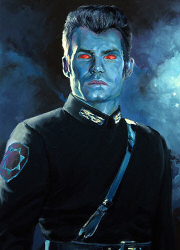
\includegraphics[height=200pt]{_img/dos-au-muur/garan-keggle.png}
\end{figure}
\vspace{-1\baselineskip}
\subsubsection{Background}
Officier supérieur dans l'armée de l'empire, Garan Keggle dirige les recherches d'artéfacts Sith pour le compte de l'empereur et son second Dark Vador. Suite à des informations sur le Talisman de Muur, il a dépéché un vaisseau de l'Insdustrial Automaton pour récupérer l'artéfact sur Taris sous couvert de projet scientifique.

Son contact chez IA est \nameref{sec:vyna-anen}, de manière générale Garan n'a que très peu de contact avec ses sous-traitant pour éviter que les ennuis remontent jsuqu'à l'empire. 

Garan est un home déterminé et sans pitié, initié au coté obscur de la Force, il attend la première occasion pour se débarrasser de ses rivaux et pouvoir prétendre au plus vite à la place d'apprenti et plus tard de seigneur Sith.

\subsubsection{Traits}
\begin{itemtable}[ c c c c c ]
    \textbf{Agi} & \textbf{Int} & \textbf{\^Ame} & \textbf{For} & \textbf{Vig} \\
    d6           & d10          & d10            & d6           & d8           
\end{itemtable}
\begin{itemtable}[ l X ]
    \textbf{Allure}      & 6 \\
    \textbf{Compétences} & Intimidation d10, Tir d10, Combat d8, Maitrise Force d8, Perception d6 \\
    \textdb{Atouts}      & Commandement, Grande aura de commandement
\end{itemtable}

\subsubsection{Défense}
\begin{itemtable}[ c c ]
    \textbf{Parade}     & \textbf{Résistance} \\
    6                   & 6 
\end{itemtable}

\newpage
\subsection{Gil Harend}  \label{sec:gil-harend}
\begin{figure}[h!]
    \centering
    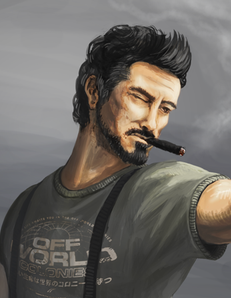
\includegraphics[height=200pt]{_img/dos-au-muur/gil-harend.png}
\end{figure}
\subsubsection{Background}
Double background selon la voie choisie.

Gil Harend est un père qui essai tant bien que mal d'élever sa fille de 16 ans, Abygaelle, dans les bas fonds de Taris. Depuis la disparition se sa femme Karie, la vie est très difficile. De plus les contrebandiers font régulièrement des razzia dans leur village pour kidnapper les jeunes filles et les revendre comme esclaves. Il y a deux jours, c'est Abygaelle qui a été enlevée. Gil fera tout pour la retrouver.\\

Gil Harend est un contrebandier qui opère dans les bas fonds de Taris. Avec ses 3 accolytes Gil fait des petits boulots plus ou moins légaux mais ce qui rapporte le plus c'est la revente de jeunes esclaves. Il y a 2 jours, lui est son équipe on kidnappés une jeune fille de 16 ans dans un village des bas fonds.

\subsubsection{Traits}
\begin{itemtable}[ c c c c c ]
    \textbf{Agi} & \textbf{Int} & \textbf{\^Ame} & \textbf{For} & \textbf{Vig} \\
    d4           & d8           & d4             & d8           & d8           
\end{itemtable}
\begin{itemtable}[ l X ]
    \textbf{Allure}      & 6 \\
    \textbf{Compétences} & Tir d6, Combat d4, Persuasion d6
\end{itemtable}

\subsubsection{Défense}
\begin{itemtable}[ c c ]
    \textbf{Parade}     & \textbf{Résistance} \\
    4                   & 6 
\end{itemtable}

\newpage
\subsection{Pulsipher} \label{sec:pulsipher}
\begin{figure}[h!]
    \centering
    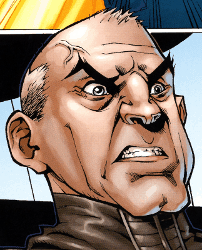
\includegraphics[height=200pt]{_img/dos-au-muur/pulsipher.png}
\end{figure}

\subsubsection{Background}
Pulsipher est un Mandalorien qui vécut plus de 3000 ans avant l'avènement de l'empire. Scientifique Néo-Croisé, il s'intéressait à la Force et tout ce qui s'y rattache. Il était persuadé que le secret de la Force lui permettrait de mettre fin à la guerre. 

C'est lui qui découvrit dans les bas-fonds de Taris et qui le ramena sur Jebble.

\subsubsection{Traits}
\begin{itemtable}[ c c c c c ]
    \textbf{Agi} & \textbf{Int} & \textbf{\^Ame} & \textbf{For} & \textbf{Vig} \\
    d4           & d12          & d4             & d8           & d6           
\end{itemtable}
\begin{itemtable}[ l X ]
    \textbf{Allure}      & 6 \\
    \textbf{Compétences} & Tir d8, Combat d8, Persuasion d6, Connaissance d12
\end{itemtable}

\subsubsection{Défense}
\begin{itemtable}[ c c ]
    \textbf{Parade}     & \textbf{Résistance} \\
    6                   & 8 
\end{itemtable}

\newpage
\subsection{Lucy} \label{sec:lucy-pher}
\begin{figure}[h!]
    \centering
    
\includegraphics[height=200pt]{_img/dos-au-muur/lucy.png}
\end{figure}

\subsubsection{Background}
Lucy est une IA particulièrement avancée (même pour la période du JdR). Mise au point par Pulsipher lui-même a partir d’un modèle de base, elle est la gardienne du Laboratoire et de tout se qu’il renferme. \'A l’époque où le labo était en activité, Lucy prenait en charge la plupart des caculs à effectuer sur l’ensemble des recherches. Elle était même capable d’anticiper certains résultats et d’ajuster les expériences de manière proactive.

Elle possède un plein accès au laboratoire, et par un réseau de caméra elle peut tout y voir.

\subsubsection{Traits}
\begin{itemtable}[ c c c c c ]
    \textbf{Agi} & \textbf{Int} & \textbf{\^Ame} & \textbf{For} & \textbf{Vig} \\
    d0           & d12+4        & d0             & d0           & d8           
\end{itemtable}
\begin{itemtable}[ l X ]
    \textbf{Allure}      & 0 \\
    \textbf{Compétences} & Tir d10, Combat d0, Persuasion d10, Connaissance d12
\end{itemtable}

\subsubsection{Défense}
\begin{itemtable}[ c c ]
    \textbf{Parade}     & \textbf{Résistance} \\
    0                   & 6 
\end{itemtable}

\newpage
\subsection{Céleste Morne*} \label{sec:celeste-morne}
\begin{figure}[h!]
    \centering
    
\includegraphics[height=200pt]{_img/dos-au-muur/celeste-morne.png}
\end{figure}

\subsubsection{Background}
Issue d’une famille de Jedi établie à Ossus, elle perdie tout ce qu’elle avait quand les Siths dévastèrent la planète durant la grande guerre des Siths. Sous la tutelle de Krynda Draay elle fut formée aux arts Jedi et, après une formation d’Ombre Jedi, elle fut recruté par le Covenant.

C’est en tant qu’Ombre du Covenant qu’elle partie en mission pour retrouver le Talisman de Muur et qu’elle croisa la route de \nameref{sec:pulsipher}. Lors de sa tentative pour sauver ce dernier et pour récupérer l’artéfact, celui-ci, attiré par les pouvoir de Céleste pris possession de son corps. Céleste parveint à le maitriser juste assez longtemps pour que Zayne Carrick, son apprenti l’enferme dans l’\nameref{sec:oubliette-de-dreypa}.

\subsubsection{Traits}
\begin{itemtable}[ c c c c c ]
    \textbf{Agi} & \textbf{Int} & \textbf{\^Ame} & \textbf{For} & \textbf{Vig} \\
    d10          & d8           & d10            & d6           & d8           
\end{itemtable}
\begin{itemtable}[ l X ]
    \textbf{Allure}      & 0 \\
    \textbf{Compétences} & Tir d6, Combat d12, Persuasion d10, Maitrise de la force d12
\end{itemtable}

\subsubsection{Défense}
\begin{itemtable}[ c c ]
    \textbf{Parade}     & \textbf{Résistance} \\
    8                   & 6 
\end{itemtable}

\newpage
\subsection{Fane Peturri} \label{sec:fane-peturri}
\begin{figure}[h!]
    \centering
    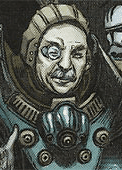
\includegraphics[height=200pt]{_img/dos-au-muur/fane-peturri.png}
\end{figure}

\subsubsection{Background}
Fane Peturri était un historien qui vécut durant les derniers décennies de la République et au tout début de l'Empire. Il semble qu'il était également un vieil ami de Palpatine et un des rares à savoir que celui-ci était un Seigneur Sith, ce qui fit qu'il eut des liens étroits avec l'Empire dès sa proclamation.

\subsubsection{Traits}
\begin{itemtable}[ c c c c c ]
    \textbf{Agi} & \textbf{Int} & \textbf{\^Ame} & \textbf{For} & \textbf{Vig} \\
    d6           & d10          & d4             & d6           & d8           
\end{itemtable}
\begin{itemtable}[ l X ]
    \textbf{Allure}      & 6 \\
    \textbf{Compétences} & Tir d4, Réseau d10, Connaissance (Empire) d10, Connaissance (Sith) d10
\end{itemtable}

\subsubsection{Défense}
\begin{itemtable}[ c c ]
    \textbf{Parade}     & \textbf{Résistance} \\
    4                   & 6 
\end{itemtable}

\newpage
\subsection{Schurk-Heren}\label{sec:schurk-heren}
\begin{figure}[h!]
    \centering
    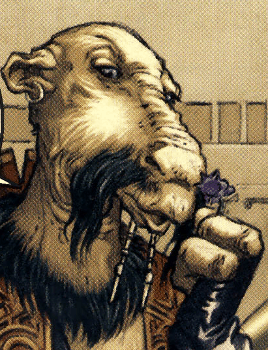
\includegraphics[height=200pt]{_img/dos-au-muur/pnjs/schurk-heren.png}
\end{figure}

\newpage
\subsection{Dass Jennir} \label{sec:dass-jennir}
\begin{figure}[h!]
    \centering
    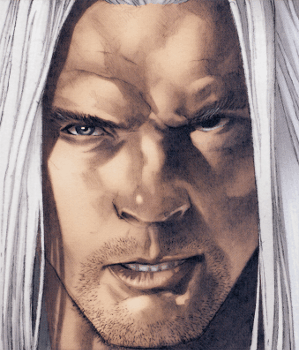
\includegraphics[height=200pt]{_img/dos-au-muur/pnjs/dass-jennir.png}
\end{figure}

\newpage
\subsection{Queen Jool} \label{sec:queen-jool}
\begin{figure}[h!]
    \centering
    
\includegraphics[height=200pt]{_img/dos-au-muur/pnjs/queen-jool.png}
\end{figure}
	\section{Bestiaire}

\subsection{Rakghoul}
\label{sec:rakghoul}
\noindent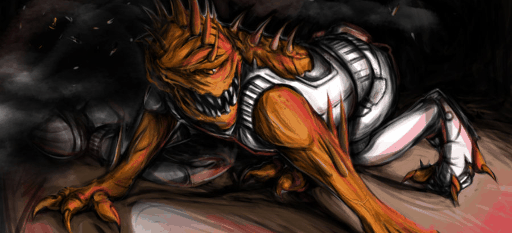
\includegraphics[width=\linewidth]{_img/dos-au-muur/rakghoul.png}

\subsubsection{Traits}

\begin{itemtable}[ c c c c c ]
    \textbf{Agi} & \textbf{Int} & \textbf{\^Ame} & \textbf{For} & \textbf{Vig} \\
    d8           & d6           & d6             & d8           & d8
\end{itemtable}
\begin{itemtable}[ l X ]
    \textbf{Allure}      & 6 \\
    ~                    & Vision Nocturne \\
    ~                    & Marche sur les murs \\
    \textbf{Compétences} & Combat d8, Discrétion d6
\end{itemtable}

\subsubsection{Défense}
\begin{itemtable}[ c c ]
    \textbf{Parade}     & \textbf{Résistance} \\
    6                   & 6 
\end{itemtable}

\subsubsection{Attaque}
\begin{itemtable}[ X c c ]
    ~       & \textbf{Combat}   & \textbf{Dégats} \\
    Griffes & d8                & 1d6 
\end{itemtable}

\newpage
\subsubsection{Background}
Les Rakghouls sont une espèce issue d’une maladie créée par le seigneur Sith Karness Muur. Les individus atteint par cette maladie deviennent des monstres incapables de penser par eux-mêmes. Karness peut les contrôler grâce à son talisman (Le Talisman de Muur).

La maladie se transmet par une griffure ou une morsure mais cela ne fonctionne pas avec les êtres sensibles à la Force. Karness a créé ce virus à partir du coté Obscur de la Force ce qui explique une forte présence obscure près de ces monstres.

Karness a créé plusieurs versions du virus car les premiers Rakghouls ne répondaient pas bien au contrôle de Karness. Les nouveaux sont plus réceptifs et plus fort.

Quand le Talisman de Muur a été perdu dans les bas fonds de Taris, on a peu constaté que les créatures, suite à une exposition prologée au Talisman finissaient par se transformer en Rakghouls. Mais les Rakghouls transformé de cette façon sont bestiaux, stupides et sans âme. Ils attaquent tout ce qui bouge. Ces créatures ne fonctionnent qu’à l’instinct.

\clearpage
\subsection{Rakghoul Amblyope}
\label{sec:rakghoul-amblyope}
\noindent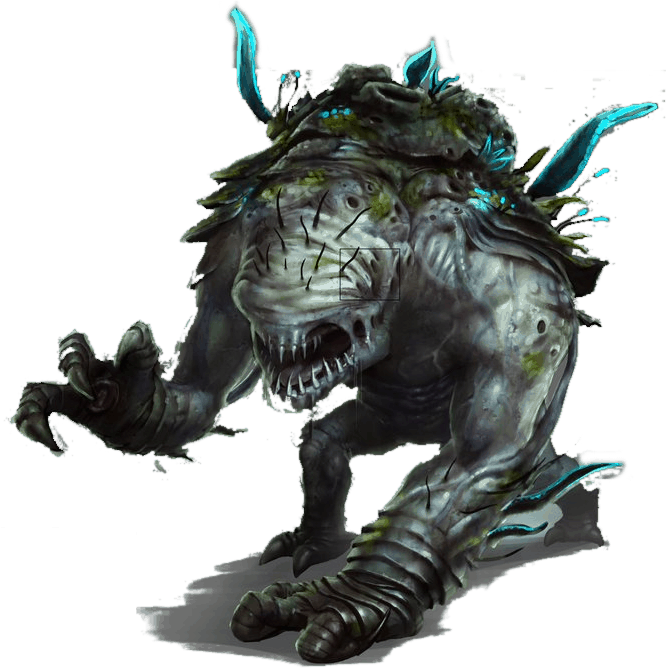
\includegraphics[width=\linewidth]{_img/dos-au-muur/rakghoul-amblyope.png}

\subsubsection{Traits}

\begin{itemtable}[ c c c c c ]
    \textbf{Agi} & \textbf{Int} & \textbf{\^Ame} & \textbf{For} & \textbf{Vig} \\
    d4           & d6           & d6             & d12+2        & d10
\end{itemtable}
\begin{itemtable}[ l X ]
    \textbf{Allure}      & 5 \\
    \textbf{Taille}      & +5 \\
    ~                    & Vision de Force \\
    ~                    & \'Enorme (+2 pour les jets d’attaque adverses)\\
    \textbf{Compétences} & Combat d10
\end{itemtable}

\subsubsection{Défense}
\begin{itemtable}[ c c ]
    \textbf{Parade}     & \textbf{Résistance} \\
    5                   & 12 
\end{itemtable}

\subsubsection{Attaque}
\begin{itemtable}[ X c c ]
    ~           & \textbf{Combat}   & \textbf{Dégats} \\
    Mains nues  & d10               & d12+2 
\end{itemtable}

\newpage
\subsubsection{Background}
Version stéroïdée des Rakghouls standard, Amblyope est notre petit boss de niveau.

Quand les Rakghouls sont livrés à eux-mêmes et qu’ils laissent libre cours à leurs plus bas instincts, il arrive qu’un Rakghoul plus fort que les autres s’en prenne à ces petits camarades et les dévore sans scrupules. Cet afflux de Force Obscure peut le faire muter et le Rakghoul devient une espèce de gros monstre de 3m de haut, complètement aveugle mais attiré par les émanations de Force, il attaque machinalement les adversaires les plus sensibles à la Force. 

\clearpage

\subsection{Contrebandier (Taris)} \label{sec:taris-contrebandier}
\noindent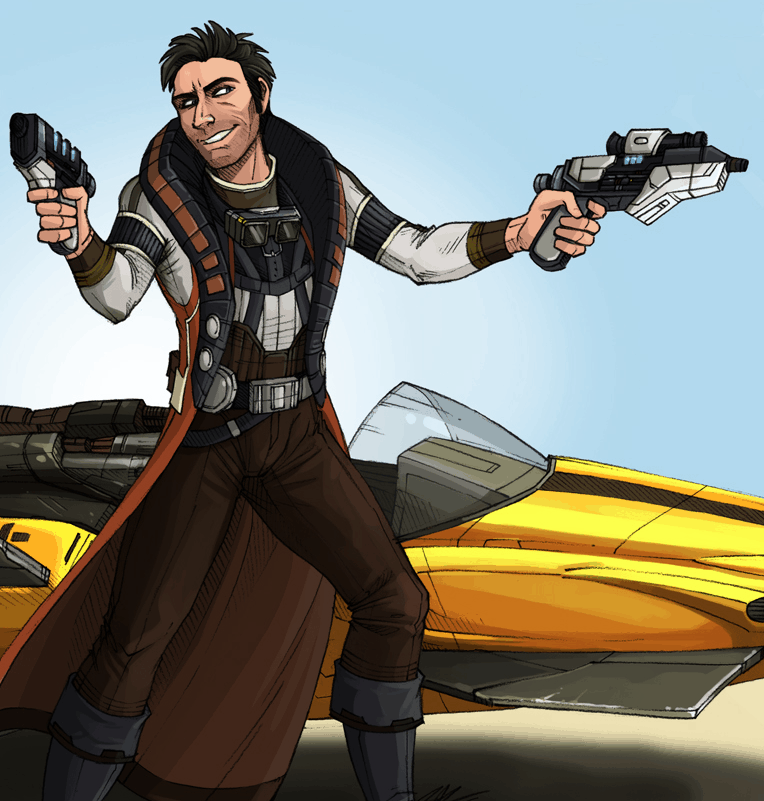
\includegraphics[width=\linewidth]{_img/dos-au-muur/contrebandier.png}

\subsubsection{Traits}

\begin{itemtable}[ c c c c c ]
    \textbf{Agi} & \textbf{Int} & \textbf{\^Ame} & \textbf{For} & \textbf{Vig} \\
    d6           & d6           & d4             & d8           & d8
\end{itemtable}
\begin{itemtable}[ l X ]
    \textbf{Allure}      & 6 \\
    \textbf{Compétences} & Combat d8, Tir d10
\end{itemtable}

\subsubsection{Défense}
\begin{itemtable}[ c c ]
    \textbf{Parade}     & \textbf{Résistance} \\
    5                   & 6 (+1)
\end{itemtable}

\subsubsection{Attaque}
\begin{itemtable}[ X c c ]
    ~           & \textbf{Combat}   & \textbf{Dégats} \\
    Blaster     & -                 & 2d6+1
\end{itemtable}

\newpage
\subsubsection{Background}
Les bas-fonds de Taris grouillent de toutes sortes de malfrats. C’est un des coins favoris de contrebandiers qui peuvent y kidnapper de jeunes enfants en toute impunité. Personne ne viendra se plaindre de la disparition d’une vermine de plus dans les bas fond.

Ce ne sont en général que des débutants attiré par la facilité. Seul ils ne représentent pas un grand danger, mais ils se promènent souvent en groupe.

\clearpage

\subsection{Storm Trooper} \label{sec:storm-trooper}
\noindent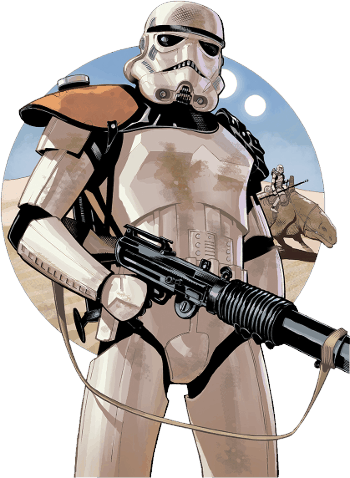
\includegraphics[width=\linewidth]{_img/dos-au-muur/stormtrooper.png}
\newpage
\subsubsection{Traits}

\begin{itemtable}[ c c c c c ]
    \textbf{Agi} & \textbf{Int} & \textbf{\^Ame} & \textbf{For} & \textbf{Vig} \\
    d4           & d6           & d4             & d8           & d8
\end{itemtable}
\begin{itemtable}[ l X ]
    \textbf{Allure}      & 6 \\
    \textbf{Compétences} & Combat d10, Tir d10
\end{itemtable}

\subsubsection{Défense}
\begin{itemtable}[ c c ]
    \textbf{Parade}     & \textbf{Résistance} \\
    7                   & 6 (+4)
\end{itemtable}

\subsubsection{Attaque}
\begin{itemtable}[ X c c ]
    ~              & \textbf{Combat}   & \textbf{Dégats} \\
    Fusil Blaster  & -                 & 2d8 (3)
\end{itemtable}

\subsubsection{Background}
Soldats dévoué de l’empire. Certain sont des clones restant de la guerre des clones d’autres non. Ils sont entrainés au combat, équipé d’une bonne armure et armé de Fusil Blaster efficaces.

\clearpage
\subsection{Wampa} \label{sec:wampa}

\clearpage
\subsection{Cybercleps} \label{sec:cybercleps}

	\onecolumn
	\nocite{*}
	\printbibliography
\end{document}